% Данный файл распространяетсяя под лицензией CC BY 4.0. Текст лицензии размещён на https://creativecommons.org/licenses/by/4.0/
% (c) Кафедра системного программирования, 2025

\documentclass[a4paper]{article}

\usepackage[a4paper, top=8mm, bottom=8mm, left=8mm, right=8mm]{geometry}

\usepackage{polyglossia}
\setdefaultlanguage[babelshorthands=true]{russian}
\setotherlanguage{english}

\usepackage{fontspec}
\setmainfont{FreeSerif}
\newfontfamily{\russianfonttt}[Scale=0.7]{DejaVuSansMono}

\usepackage[tiny, compact]{titlesec}

\usepackage{titling}
\setlength{\droptitle}{-1cm}
\pretitle{\begin{center}\begin{bfseries}\Large}
\posttitle{\par\end{bfseries}\end{center}}
\preauthor{\begin{center}\normalsize}
\postauthor{\par\end{center}\vspace{-1.8cm}}

\usepackage{hyperref}
\usepackage{bookmark}
\usepackage{csquotes}
\usepackage{graphicx}
\usepackage{float}
% Сюда можно дописывать нужные вам пакеты.

\title{Архиватор на базе Алгоритма Хаффмана}

\author{Тайманов Балкан Мередович}

% Дата много места занимает, её лучше не указывать.
\date{}

\begin{document}
\sloppy
\maketitle

\begin{flushright}
    Группа: \emph{25.Б73-мм}

    Кафедра: \emph{кафедра системного программирования}

    % Степень/звание и должность научника мы лучше вас знаем, их можно не указывать.
    Научный руководитель: \emph{Литвинов Юрий Викторович}
    
    Номер семестра практики: \emph{2}
\end{flushright} 

\section{Введение}

Алгоритм Хаффмана --- один из алгоритмов сжатия данных без потерь, предложенный Дэвидом Хаффманом в 1952 году. Идея алгоритма состоит в том, что символы, встречающиеся чаще, получают более короткий код, а редкие символы более длинный. Благодаря этому общий размер закодированных данных уменьшается. Важным свойством алгоритма является префиксность кодов: ни один код не является началом другого.
Самостоятельная реализация архиватора позволяет глубоко разобраться в устройстве алгоритмов сжатия, а также получить практический опыт работы с битовыми операциями, структурами данных и низкоуровневым управлением памятью.

\section{Постановка задачи}

\textbf{Целью работы является} реализация консольного архиватора файлов на основе алгоритма Хаффмана.

В ходе работы необходимо решить следующие задачи.

\begin{enumerate}
    \item Реализация необходимых структур данных: бинарное дерево и минимальная куча.
    \item Реализация алгоритма сжатия файлов на основе алгоритма Хаффмана.
    \item Реализация алгоритма разжатия файлов.
    \item Написание модульных и интеграционных тестов для проверки корректности работы.
    \item Проведение экспериментов по измерению степени сжатия и скорости работы на файлах различных типов и размеров.
\end{enumerate}
Результатом работы является готовый консольный инструмент, позволяющий сжимать и разжимать произвольные файлы.

\section{Описание предлагаемого решения}

Для реализации архиватора был выбран язык программирования C. Данный выбор обусловлен желанием реализовать все компоненты с нуля, без использования высокоуровневых абстракций, а также возможностью работы напрямую с памятью и битовыми операциями, что особенно важно при побитовом кодировании данных.

\subsection*{Алгоритм сжатия}

Сжатие файла выполняется в несколько этапов. На первом этапе файл читается побайтово и подсчитываются частоты встречаемости каждого байта. Результатом является массив из 256 элементов, где индекс это значение байта, а значение --- его частота.

На втором этапе из полученных частот строится минимальная куча. Использование кучи обеспечивает эффективное построение дерева Хаффмана за $O(n \log n)$. Каждый элемент кучи --- узел дерева, содержащий символ и его частоту.

На третьем этапе строится дерево Хаффмана. На каждой итерации из кучи извлекаются два узла с минимальными частотами, из них создаётся новый родительский узел с частотой равной сумме частот детей, который добавляется обратно в кучу. Процесс повторяется до тех пор, пока в куче не останется один узел --- корень дерева Хаффмана.

После построения дерева генерируется таблица префиксных кодов обходом дерева в глубину (DFS). При переходе к левому ребёнку к текущему коду добавляется бит 0, при переходе к правому --- бит 1. Когда алгоритм доходит до листа, накопленная последовательность битов становится кодом соответствующего символа.

Затем входной файл читается повторно, и каждый байт заменяется его кодом из таблицы. Биты накапливаются в буфере размером один байт. Как только буфер заполняется, он записывается в выходной файл и обнуляется. В начало сжатого файла записывается таблица частот --- масcив из 256 значений типа \texttt{size\_t}, необходимых для восстановления дерева при разжатии.

\subsection*{Алгоритм разжатия}

Разжатие начинается с чтения заголовка сжатого файла --- таблицы частот. Таблица частот была выбрана для хранения в заголовке намеренно: из неё можно восстановить дерево Хаффмана, а из дерева --- таблицу кодов. Это более компактно чем хранить саму таблицу кодов.

По таблице частот восстанавливается куча и дерево Хаффмана. Затем оставшиеся данные файла читаются побайтово. Каждый байт обрабатывается побитово: бит 0 означает переход к левому ребёнку дерева, бит 1 --- к правому. Как только алгоритм доходит до листа, соответствующий символ записывается в выходной файл, и обход начинается заново с корня. Процесс продолжается до тех пор, пока не будет восстановлено исходное количество символов.

\subsection*{Инструменты и технологии}

Реализация осуществлялась с использованием следующих технологий: язык C (стандарт C99), система сборки CMake, система автоматической сборки и тестирования GitHub Actions. Для контроля качества кода используются AddressSanitizer и Valgrind. Поскольку эти два инструмента конфликтуют между собой, в CI настроены два отдельных job: первый выполняет сборку с AddressSanitizer и запускает тесты, второй собирает проект без санитайзеров и запускает Valgrind. Также используется статический анализатор cppcheck.


\subsection*{Структура проекта}

Проект разделён на независимые модули, каждый из которых отвечает за свою часть алгоритма:

\begin{itemize}
    \item \texttt{tree} --- реализация бинарного дерева. Содержит структуру узла и функции создания и освобождения дерева.
    \item \texttt{heap} --- реализация минимальной кучи. Содержит функции добавления узла, извлечения минимального элемента и освобождения памяти.
    \item \texttt{huffman\_tree} --- основная логика алгоритма. Содержит подсчёт частот, построение кучи из частот, построение дерева Хаффмана и создание таблицы кодов.
    \item \texttt{encode} --- модуль сжатия файла.
    \item \texttt{decode} --- модуль разжатия файла.
    \item \texttt{error} --- вывод сообщений об ошибках.
\end{itemize}

\section{Эксперименты}

\subsection*{Тестирование}

Для проверки корректности работы архиватора были написаны модульные и интеграционные тесты с использованием библиотеки assert. 

Модульные тесты проверяют работоспособность каждой функции алгоритма в отдельности. Для каждого теста создавались временные входные данные, которые передавались на вход функции, после чего результат сравнивался с ожидаемым. Были написаны тесты для следующих модулей: бинарное дерево, минимальная куча, подсчёт частот, построение дерева Хаффмана и генерация таблицы кодов.

Интеграционный тест проверяет работоспособность программы целиком: создаётся временный текстовый файл, выполняется сжатие и разжатие, после чего результат побайтово сравнивается с оригиналом.

\subsection*{Замеры производительности}

Замеры проводились на следующей конфигурации: процессор Intel Core i5-13500HX, 16~ГБ оперативной памяти, ОС Fedora Linux (ядро 7.0.10-100.fc43.x86\_64), компилятор GCC 15.2.1 с флагом оптимизации \texttt{-O2}.

Для исследования эффективности алгоритма были проведены эксперименты на файлах различных типов и размеров. Каждый замер выполнялся 10 раз, после чего вычислялось математическое ожидание и среднеквадратическое отклонение. Результаты приведены в табл.~\ref{tab:compression} и табл.~\ref{tab:time}, графики --- на рис.~\ref{fig:graphs}.

Для экспериментов были выбраны следующие файлы:
\begin{itemize}
    \item Большой текстовый файл (3.4 МБ) --- для проверки эффективности на типичных данных
    \item Маленький текстовый файл (14 байт) --- для проверки поведения на маленьких файлах
    \item JPEG изображение (1.3 МБ) --- уже сжатый формат
    \item ZIP архив (1.3 МБ) --- уже сжатый формат
    \item Пустой файл --- файл без данных
\end{itemize}

\begin{table}[h]
\centering
\begin{tabular}{|l|l|r|r|r|}
\hline
Файл & Тип & Оригинал & Сжатый & Степень сжатия \\
\hline
bigTXT.txt & Текст (большой) & 3.4 МБ & 1.7 МБ & 50\% \\
smallTXT.txt & Текст (маленький) & 14 Б & 2054 Б & увеличение (заголовок) \\
photo.jpg & JPEG & 1.3 МБ & 1.3 МБ & увеличение (заголовок) \\
photo.zip & ZIP & 1.3 МБ & 1.3 МБ & увеличение (заголовок) \\
empty.txt & Пустой файл & 0 Б & 2048 Б & увеличение (заголовок) \\
\hline
\end{tabular}
\caption{Результаты экспериментов}
\label{tab:compression}
\end{table}

\begin{figure}[H]
\centering
\begin{minipage}{0.32\textwidth}
    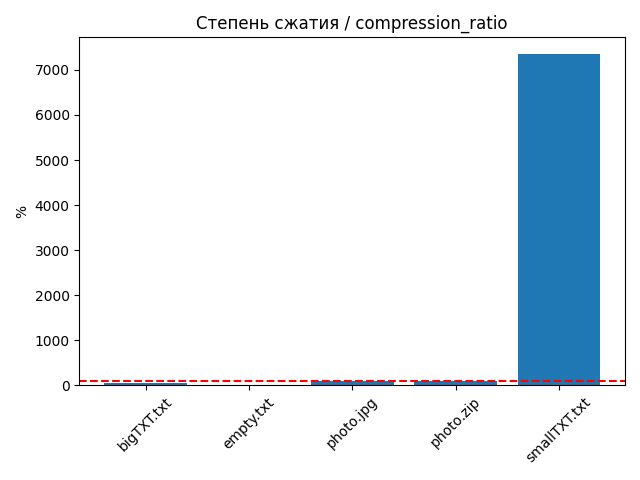
\includegraphics[width=\textwidth]{../experiments/graphs/compression_ratio.png}
\end{minipage}
\hfill
\begin{minipage}{0.32\textwidth}
    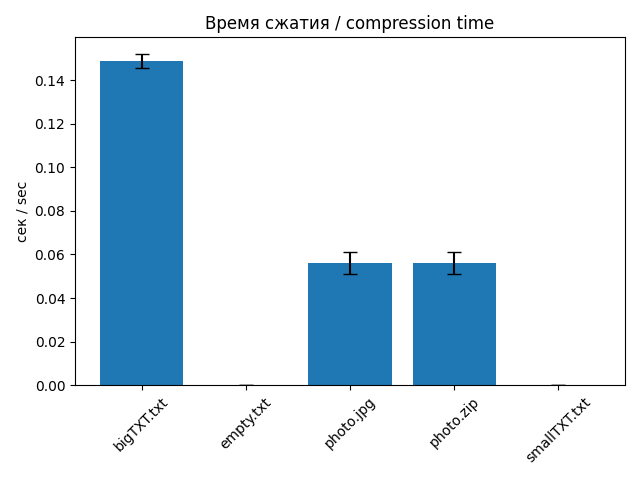
\includegraphics[width=\textwidth]{../experiments/graphs/encode_time.png}
\end{minipage}
\hfill
\begin{minipage}{0.32\textwidth}
    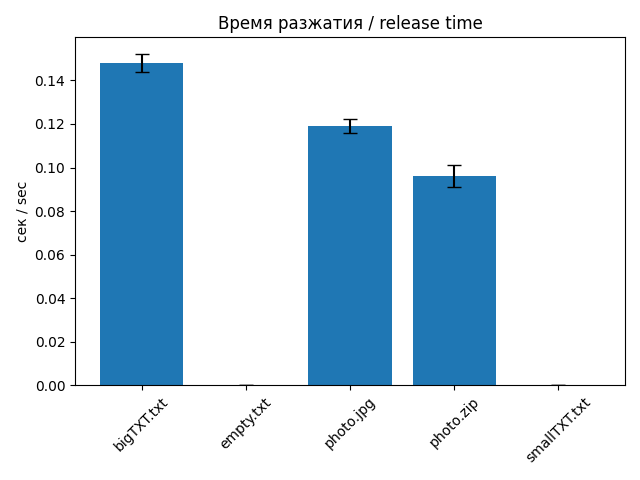
\includegraphics[width=\textwidth]{../experiments/graphs/decode_time.png}
\end{minipage}
\caption{Степень сжатия, время сжатия и время разжатия}
\label{fig:graphs}
\end{figure}

\begin{table}[h]
\centering
\begin{tabular}{|l|r|r|r|r|}
\hline
Файл & М encode (с) & σ encode & М decode (с) & σ decode \\
\hline
bigTXT.txt & 0.149 & 0.003 & 0.147 & 0.005 \\
smallTXT.txt & 0.000 & 0.000 & 0.000 & 0.000 \\
photo.jpg & 0.056 & 0.005 & 0.119 & 0.003 \\
photo.zip & 0.056 & 0.004 & 0.096 & 0.005 \\
empty.txt & 0.000 & 0.000 & 0.000 & 0.000 \\
\hline
\end{tabular}
\caption{Время работы архиватора}
\label{tab:time}
\end{table}

На рис.~\ref{fig:graphs} приведены графики степени сжатия, времени сжатия и времени разжатия.

На графике степени сжатия только большой текстовый файл показал положительный результат --- степень сжатия составила около 50\%. Для остальных файлов размер после сжатия увеличился из-за заголовка размером 2048 байт. Особенно заметно это на маленьком текстовом файле --- исходный файл (14 байт) значительно меньше заголовка.

На графике времени сжатия наибольшее время занимает большой текстовый файл (0.149~с) --- это объясняется его размером. JPEG и ZIP сжимаются примерно вдвое быстрее (0.056~с), несмотря на сопоставимый размер, поскольку их данные близки к равномерному распределению и алгоритм строит более простое дерево. Для пустого файла и маленького текстового файла время сжатия незначительно.

На графике времени разжатия картина аналогична: большой текстовый файл разжимается дольше всего (0.147~с). Интересно, что JPEG и ZIP разжимаются медленнее чем сжимаются --- это объясняется тем, что при разжатии алгоритм обходит дерево побитово для каждого символа, тогда как при сжатии достаточно табличного поиска.


\subsection*{Выводы}

Алгоритм Хаффмана показал высокую эффективность на большом текстовом файле --- степень сжатия составила около 50\%. Это ожидаемый результат, так как в текстовых файлах одни символы встречаются намного чаще других, что позволяет алгоритму хорошо их кодировать.

На уже сжатых форматах (JPEG, ZIP) алгоритм не эффективен --- размер файла почти не изменился. Это объясняется тем, что такие форматы уже используют сжатие, и распределение байтов в них близко к равномерному --- алгоритму просто нечего оптимизировать.

На маленьком текстовом файле размер после сжатия увеличился. Это происходит из-за того, что в начало сжатого файла записывается таблица частот размером 2048 байта, что значительно больше самого файла.

Пустой файл обрабатывается корректно --- записывается заголовок размером 2048 байт и завершается работа программы.

\section{Заключение}

В ходе выполнения работы получены следующие результаты:

\begin{itemize}
    \item Реализован консольный архиватор файлов на основе алгоритма Хаффмана на языке C, поддерживающий сжатие и разжатие произвольных файлов.
    \item Реализованы необходимые структуры данных: бинарное дерево и минимальная куча.
    \item Написаны модульные тесты для каждого модуля и интеграционный тест, проверяющий корректность сжатия и разжатия.
    \item Настроена автоматическая проверка кода через GitHub Actions: сборка, тесты, линтер и Valgrind.
    \item Проведены эксперименты на файлах различных типов и размеров с вычислением математического ожидания и среднеквадратического отклонения.
\end{itemize}

Репозиторий: \url{https://github.com/taymanov-bn/Huffman-archiver}

\end{document}
